\documentclass{article}
\usepackage{graphicx}
\usepackage{titletoc}
\usepackage{titlesec}
\usepackage{geometry} 
\usepackage{fontspec, xunicode, xltxtra}
\usepackage{float}
\usepackage{cite}
\usepackage{amsmath}
\usepackage{listings}
\usepackage{titletoc}
\usepackage{bm}

\geometry{left=3cm,right=3cm,top=3cm,bottom=3cm}
\DeclareMathOperator*{\argmin}{argmin}
\DeclareMathOperator*{\argmax}{argmax}
\DeclareMathOperator*{\var}{var}
\DeclareMathOperator*{\expec}{E}

\begin{document}
\title{\textsf{Homework 6 for Pattern Recognition}}
\author{Fan JIN\quad (2015011506)}
\maketitle

\section*{Question 1.1}
{
    Note that 
    $$\varepsilon_B(x) = h_B(x) - y(x) = \left[ \frac{1}{m} \sum_{i=1}^{m} {h_i(x)} \right] - y(x)$$
    $$= \frac{1}{m} \sum_{i=1}^{m} {[h_i(x) - y(x)]} = \frac{1}{m} \sum_{i=1}^{m} {\varepsilon_i(x)}.$$
    It follows that 
    $$E_{h_B} = \frac{1}{n} \sum_{j=1}^{n}{[\varepsilon_B (x_j)]^2} = \frac{1}{m^2 n} \sum_{j=1}^{n}{ \left[ \sum_{i=1}^{m}{\varepsilon_i(x_j)} \right]^2 }$$
    $$= \frac{1}{m^2 n} \sum_{j=1}^{n}{ \left[ \sum_{i=1}^{m}{(\varepsilon_i(x_j))^2} + 2 \sum_{i=1}^{m}{ \sum_{k=1, k\neq i}^{m}{\varepsilon_i(x_j) \varepsilon_k(x_j)}} \right] }$$
    $$= \frac{1}{m^2 n} \left[ \sum_{i=1}^{m}\sum_{j=1}^{n}{(\varepsilon_i(x_j))^2} + 2 \sum_{i=1}^{m}{ \sum_{k=1, k\neq i}^{m} \sum_{j=1}^{n} {\varepsilon_i(x_j) \varepsilon_k(x_j)}} \right]$$
    $$= \frac{1}{m^2 n} \left[ \sum_{i=1}^{m}\sum_{j=1}^{n}{(\varepsilon_i(x_j))^2} + 2 \sum_{i=1}^{m}{ \sum_{k=1, k\neq i}^{m} 0 } \right]$$
    $$= \frac{1}{m^2 n} \left[ \sum_{i=1}^{m}\sum_{j=1}^{n}{(\varepsilon_i(x_j))^2} \right]$$
    $$= \frac{1}{m} \frac{1}{m} \sum_{i=1}^{m} \left[ \frac{1}{n}\sum_{j=1}^{n}{(\varepsilon_i(x_j))^2} \right] = \frac{1}{m} E_h.$$
}

\section*{Question 1.2}
{
    By Cauchy Inequality, we have
    $$\left[ \sum_{i=1}^{m}{(\varepsilon_i(x_j) \cdot 1)} \right]^2 \leq \left[ \sum_{i=1}^{m}{(\varepsilon_i(x_j))^2} \right] \cdot \left[ \sum_{i=1}^{m}{1^2} \right] = m \sum_{i=1}^{m}{(\varepsilon_i(x_j))^2}.$$
    It follows that 
    $$E_{h_B} = \frac{1}{n} \sum_{j=1}^{n}{[\varepsilon_B (x_j)]^2} = \frac{1}{m^2 n} \sum_{j=1}^{n}{ \left[ \sum_{i=1}^{m}{\varepsilon_i(x_j)} \right]^2 }$$
    $$\leq \frac{1}{m^2 n} \sum_{j=1}^{n}{ \left[ m \sum_{i=1}^{m}{(\varepsilon_i(x_j))^2} \right] }$$
    $$= \frac{1}{m n} \sum_{j=1}^{n}{ \left[ \sum_{i=1}^{m}{(\varepsilon_i(x_j))^2} \right] }$$
    $$= \frac{1}{m} \sum_{i=1}^{m} \left[ \frac{1}{n}\sum_{j=1}^{n}{(\varepsilon_i(x_j))^2} \right] = E_h.$$
}

\section*{Question 2.1}
{
    \textbf{Lemma:}\quad With all weights $w_i$, $d$ and $j$ fixed, there exists $k$ such that the following quantity
    $$\sum_{i=1}^{n}{w_i 1\{ h_{a,d,j}(x_i) \neq y_i \}},$$ as a function of $a$, 
    is minimized at $a = x_{k,j}$, where $x_{k,j}$ is the $j$-th feature of the $k$-th sample.

    \textbf{Proof:}\quad This quantity, with all weights $w_i$, $d$ and $j$ fixed, is a linear combination of many sign functions $$1\{ h_{a,d,j}(x_i) \neq y_i \} $$ with respect to $a$. Therefore, it is a staircase function, which can be minimized at one of those steps. By definition, the threshold for $1\{ h_{a,d,j}(x_i) \neq y_i \} $ is $a = x_{k,j}$, and the lemma is thus proved.

    With this lemma, we only need to find the optimal $a$, $d$, $j$ from a finite set, i.e., to find $k$, $d$ and $j$ such that 
    $$a = x_{k,j} ,$$
    $$d = 1 \mathrm{\quad or\quad } d = -1 ,$$
    $$1 \leq k \leq n ,$$
    $$1 \leq j \leq p.$$
    The size of this finite set is merely $2np$.

    \textbf{Note:}\quad For this dataset, the images are nearly binary: the gray-scale values are very close to either 0 or 1. In such cases, we can speed up calculations by neglecting the repeating values in $X$, i.e., doing a ``unique'' operation. 

    \begin{table}[!hbp]
        \centering
        \begin{tabular}{|c|c|c|}
        \hline
        Iterations & Training error & Testing error \\
        \hline
        30.0000  &  0.0180  &  0.0753 \\
        \hline
        100.0000    &     0  &  0.0653 \\
        \hline
        200.0000   &      0  &  0.0598 \\
        \hline
        \end{tabular}
        \caption{Error rates through training}
    \end{table}

    \begin{figure}[H]
        \centering
        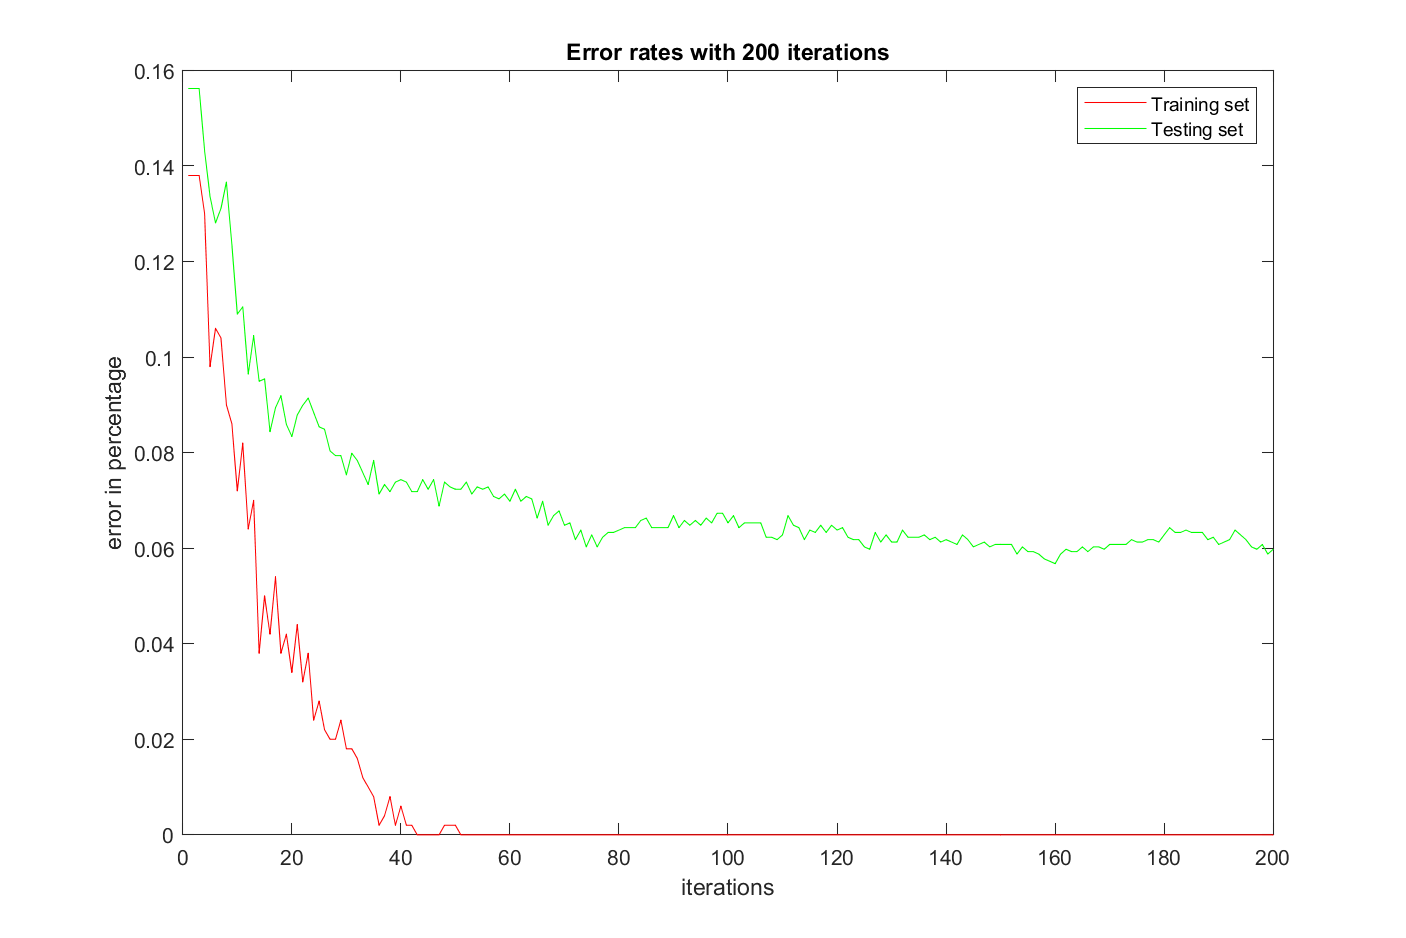
\includegraphics[width = 1\linewidth]{stump-AdaBoost/error.png}
        \caption{Error rates through training}
    \end{figure}
}

\section*{Questions 2.2 \& 2.3}
{
    Keep using 5-fold cross validation through training.

    \begin{table}[!hbp]
        \centering
        \begin{tabular}{|c|c|c|}
        \hline
        Model & Validation error & Testing error \\
        \hline
        Fine Tree  &  0.122000  &  0.084380 \\
        \hline
        Medium Tree  &   0.126000  & 0.084380 \\
        \hline
        Coarse Tree   &  0.124000  &  0.098443 \\
        \hline
        Bagged Trees 30   &    0.044000 &  0.047715 \\
        \hline
        Bagged Trees 100   &  0.038000  &  0.037670 \\
        \hline
        Bagged Trees 300   &   0.042000  & 0.035660 \\
        \hline
        \end{tabular}
        \caption{Error rates of the 6 tree models}
    \end{table}

    All 6 models have been saved to ``models.mat'' automatically. 

    For the 3 tree models, the FineTree (max division number = 4) and MediumTree (max division number = 20) give the best performance on both validation set and testing set, while the CoarseTree (max division number = 100) has much higher error rate, especially on the testing set.

    For the 3 bagged trees, it attains the lowest error rate when the number of classifiers, the hyperparamter, is tuned at 30.
}

\section*{Question 2.4}
{
    \textbf{Briefly speaking:}\quad
    ``Boosting'' and ``random forest'' are both useful workarounds to the problem that single decision trees are easily overfitting. 

    \textbf{Detailed comparison:}
    \begin{itemize}
        \item Judging from the output, ensembled models like bagged trees models attain the lowest error rate (around 4\%), the AdaBoost the medium (around 6\%), and single tree models the highest (around 12\%). This means it is possible to improve the performance by ensembling multiple models. Ensembling contributes to better performance, makes the model robust against noise, and fits paralell computation as well.

        \item The idea of boosting is useful in that it assigns weights to different samples, and allows the classifier to concentrate on the samples in which it classifies wrong. It makes the training faster, and a bit more robust. The weights and the parameters are updated iteratively. Sometimes it also employs multiple trees and makes decision by taking a vote, as shown in AdaBoost.

        \item Hyperparamter tuning is cricial to our model. This not only applies in a single decision tree (where we can adjust the max division number), but it is also seen in bagged trees (where we can adjust the number of classifiers). More divisions and more sub-classifiers do not always bring better performance, as shown in Table 2.
        
        \item It is necessary to identify overfitting. From Figure 1, we see it starts to overfit after 60 iterations. It is better to stop at 60 iterations than to continue training. 
    \end{itemize}
}

\section*{Source Code}
{
    Please download the souece code from http://39.106.23.58/files/PR6\_2015011506.7z

    For Question 2, please run ``main.m''. It may take \emph{less than a minute} to train the network, but the result is reproducible because of the random seed.

    For each model, I clicked ``Generate code'' button to transcript my operations into MATLAB codes, and stored each of them in the corresponding ``.m'' file. These files include:
    \begin{itemize}
        \item trainClassifierFineTree.m
        \item trainClassifierMediumTree.m
        \item trainClassifierCoarseTree.m
        \item trainClassifierBaggedTrees\_30.m
        \item trainClassifierBaggedTrees\_100.m
        \item trainClassifierBaggedTrees\_300.m
    \end{itemize}
    Thus, the steps above can be easily reproduced without using the GUI of the toolbox. 

}

\clearpage
\end{document}
    